% Draft of 31 October 2026. Hand-written LaTeX (not generated by build_latex.py).
% Layout: IEEE conference template, as specified by the supervisor.
% Citations: author-year (natbib + plainnat), as requested by the supervisor.
\documentclass[conference]{IEEEtran}
\usepackage[T1]{fontenc}
\usepackage[utf8]{inputenc}
\usepackage{microtype,graphicx,booktabs,tabularx,amsmath,amssymb}
\usepackage[authoryear,round]{natbib}
\usepackage[hidelinks]{hyperref}
\graphicspath{{figures/}}
\setlength{\emergencystretch}{2em}
\newcolumntype{R}{>{\raggedleft\arraybackslash}X}

\title{Comparing Behavioural Cloning, DAgger and GAIL for RoboCup Walking:\\
Comparisons Across Training Resource Allocations}

\author{\IEEEauthorblockN{Author name to be supplied}
\IEEEauthorblockA{School and institution to be supplied\\
Email to be supplied}}

\begin{document}
\maketitle

\begin{abstract}
Behavioural cloning (BC), dataset aggregation (DAgger) and generative adversarial imitation learning (GAIL) differ in their use of expert demonstrations, expert queries, environment interaction and optimization. We compare these methods on simulated humanoid walking in the RoboCup 3D league, imitating the FC Portugal walking controller through its native gait interface. Across 3,205 unique 60-second deployments in several evaluation cohorts, with comparisons paired on shared rounds, we measure task progress, imitation fidelity and mechanical stability on the original field and on fields with altered surface slip. Every supervised-initialized learner's mean progress was within 1.8\% of the expert's, while untrained networks and zero actions driving the same gait engine made no forward progress. The fidelity ranking, however, depends on which resource is held fixed: DAgger has 7.2$\times$ lower action error at the initial fixed budgets, BC is 33.3\% lower at matched optimizer updates, and DAgger is 17.7\% lower under a common validation-stopping rule while using 66.3\% more updates. On altered surfaces BC's 4--11$\times$ fidelity deficit shrinks to 0.9--1.1$\times$ with further fitting. A first GAIL implementation diverged; after changes to its reward and update rules, GAIL refinement changed its initializer's held-out action error by $-0.05$\% (BC initializer) and $+2.4$\% (DAgger initializer). These results concern one walking task, a shared gait interface and the tested training allocations; they do not identify a general algorithm ranking. We recommend that comparisons of imitation methods state which resource they standardise and report results under more than one standardisation.
\end{abstract}

\begin{IEEEkeywords}
imitation learning, behavioural cloning, DAgger, GAIL, humanoid locomotion, RoboCup, experimental design
\end{IEEEkeywords}

%======================================================================
\section{Introduction}

RoboCup teams develop low-level skills such as walking and kicking by hand engineering and by optimization, including reinforcement learning \citep{ingram2023,beukman2024,abreu2025}. Imitation learning offers a way to train a policy from such an existing controller. We consider three methods. Behavioural cloning (BC) fits expert actions by supervised learning. DAgger queries the expert at states the learner itself visits, to correct the compounding errors that follow when a cloned policy drifts away from the demonstrations \citep{ross2011}. GAIL matches the expert's state--action distribution through an adversarially learned reward and reinforcement learning \citep{ho2016}. \citet{ho2016} motivate GAIL by noting that BC ``only tends to succeed with large amounts of data, due to compounding error caused by covariate shift'' \citep{ho2016}.

\citet{spencer2021} report that how much interaction helps depends on the setting. A comparison is also shaped by how resources are allocated, because the three methods do not consume the same resources. BC uses expert demonstrations and supervised optimization. DAgger adds expert queries at learner-visited states and repeated refitting of a growing dataset. GAIL requires environment interaction and actor--critic and discriminator optimization, in addition to its initialization costs. Our comparisons control selected resources; they do not equalize all costs.

We study this in the RoboCup 3D simulation league, imitating the walking controller of the FC Portugal team \citep{abreu2025} on a simulated NAO humanoid. We ask three questions:
\begin{itemize}
\item \textbf{RQ1 (stability):} do BC, DAgger and GAIL differ in fall rate and kinematic smoothness while walking usefully?
\item \textbf{RQ2 (efficiency):} how do imitation fidelity and task performance vary across the tested allocations of expert labels, environment interaction and optimization?
\item \textbf{RQ3 (expert comparison):} how close are the learners to the expert in progress and velocity, and does closer imitation improve these outcomes?
\end{itemize}
We additionally test the learners on fields with altered surface slip, and whether providing the slip value as an input changes the measured outcomes.

Our contributions are as follows. (i) A comparison of the three methods across 3,205 unique deployments, paired within shared evaluation cohorts, with controls testing whether zero actions or untrained networks produce useful walking through the gait engine. (ii) Measurements showing that the BC--DAgger fidelity ranking reverses twice across three standardisations of resources, while observed mean progress remains close to the expert under all three. (iii) A record of the changes made to GAIL after a first implementation diverged, and of the resulting behaviour: the changed method alters its initializer's held-out action error by at most 2.4\%. (iv) An assessment of the scope of these comparisons and recommendations for reporting resource allocations.

%======================================================================
\section{Background}

\subsection{Distribution shift and when interaction helps}
\citet{pomerleau1989} observed that a cloned driving network ``must not solely be shown examples of accurate driving, but also how to recover''. \citet{ross2011} formalized the problem: a policy trained only on expert states can encounter states the expert never visited, and its errors can compound over the horizon. DAgger aggregates expert labels at learner-visited states. Its analysis relates policy performance to supervised loss under the assumptions of the no-regret reduction \citep{ross2011}. Supervised fitting error is therefore relevant when comparing trained policies. Second, the cost of a mistake depends on how quickly the system can recover: if the expert returns to its normal state distribution within a few steps, the relevant constant ``will be $O(1)$'' rather than growing with the horizon \citep[\S2.2]{ross2011}.

\citet{spencer2021} distinguish regimes of covariate shift. In the simplest, the expert is realizable by the learner's policy class, and they report that commonly used benchmarks ``are well solved by naive behavioral cloning'' in this regime. \citet{celemin2022} evaluate the data efficiency of interactive methods as ``the amount of human data (i.e., feedback) that is required''.

\subsection{Adversarial imitation}
GAIL trains a discriminator to separate expert and policy state--action pairs and uses its output as a reward for policy optimization \citep{ho2016}. Its original evaluation used trust-region updates and suggested ``initializing policy parameters with behavioral cloning'' to reduce environment interaction. For generative adversarial networks, \citet{goodfellow2014} note that the minimax objective saturates early in training, when the discriminator rejects generated samples with high confidence, and propose a non-saturating alternative. Using it changes what is being minimized, so its optimization objective should not be identified uncritically with the original minimax divergence objective \citep{jolicoeur2018}. \citet{orsini2021} show that adversarial imitation is highly sensitive to such implementation choices, including input normalization, reward form and the handling of episode termination, and that BC pretraining gives little benefit in most of their environments.

\subsection{Resource allocation in published comparisons}
Published comparisons fix resources in different ways. \citet{ho2016} gave the adversarial and apprenticeship methods ``exactly the same amount of environment interaction'' but trained their BC baseline ``until validation error stops decreasing''. \citet{ross2011} plot performance against the number of training labels collected. These reported comparisons use different resource measures. \citet{codevilla2019} report that behaviour-cloning results are sensitive to initialization and data order, and report means over repeated runs because their simulator is non-deterministic. \citet{hussenot2021} show that the choice of validation criterion itself affects which imitation policy is selected.

\subsection{RoboCup 3D}
The RoboCup 3D league simulates NAO humanoids in the rcssserver3d simulator. RobocupGym exposes such tasks for reinforcement learning, with baselines trained for millions of steps \citep{beukman2024}. \citet{ingram2023} report that a kicking agent penalized for falling learned to stand still, so a low fall count accompanied no task progress.

%======================================================================
\section{Methods}

\subsection{Task, expert and policy interface}
The expert is the unchanged FC Portugal walking controller \citep{abreu2025}. At each 20\,ms step it maps 63 observation features (body state and target information) to 16 native gait actions. A stateful gait generator and inverse kinematics convert those actions into joint commands for the robot's 22 joints. Every learner uses the same interface: a $63\!\rightarrow\!256\!\rightarrow\!256\!\rightarrow\!16$ ReLU network producing the 16 gait actions. The expert network is smaller than the learners (one 64-unit tanh hidden layer). Policies that receive surface information take one extra normalized slip input (64 inputs). The gait generator and inverse kinematics are identical for the expert and all learners.

Each episode walks towards a sequence of targets inside one half of the field. A fall is detected when head height drops below a threshold or the torso tilts beyond $60^\circ$ in roll or pitch, and triggers a common reset and stabilization. Reset time is excluded from the 3,000 active steps (60\,s) of each deployment, so fall counts measure detected balance losses rather than autonomous recovery.

\subsection{Learners}
\label{sec:learners}
\textbf{BC} trains on 170,000 expert state--action pairs (balanced long-walk and short-turn episodes), with separate 10,000-example validation and test sets, using Adam (learning rate $10^{-4}$, batch 256) and mean squared error over the 16 actions.

\textbf{DAgger} starts from a policy fitted on 100,000 balanced expert examples, then performs seven rounds. Each round collects 10,000 steps in which the expert controls the robot with probability $\beta$ (schedule 0.8, 0.6, 0.4, 0.2, 0, 0, 0) and otherwise the learner does; the expert labels every visited state; the policy is refitted on the full aggregate for 50 epochs. The final aggregate has 170,000 labels, the same number as BC's training set, but 70,000 are labels collected during the expert--learner mixture rollouts (learner-only in the final three rounds).

\textbf{GAIL} uses the 170,000 expert examples as the expert distribution and a PPO actor--critic \citep{schulman2017} trained on 70,000 learner environment steps. We report two supervised-initialized variants, GAIL-BC and GAIL-DM (initialized from BC and from DAgger respectively), and one random-initialized control. A first implementation with the minimax reward $-\log(1-D)$ diverged (Section~\ref{sec:gail}). The final recipe uses the non-saturating reward $r(s,a)=\log D(s,a)$ \citep{goodfellow2014}, discriminator inputs normalized by expert statistics, 0.9/0.1 label smoothing, an interpolation gradient penalty, discriminator early stopping once both class accuracies exceed 0.95, an actor learning rate 100 times smaller than the critic's, target-KL early stopping with rollback of over-large updates, and a decaying auxiliary BC loss that anchors the actor to its initializer. We therefore describe this method as BC-anchored GAIL refinement; our conclusions concern this recipe.

\subsection{Surfaces and training stages}
The original field is kept as installed. Altered surfaces set a single contact-slip scalar for the whole field (an early setter that appeared to change slip did not, and was replaced; Section~\ref{sec:measurement}). Training on varied surfaces cycles through slip values 0.025, 0.1, 0.2, 1 and 10. \emph{Continued} models start from the corresponding original-field model; \emph{varied-only} models are trained on varied surfaces from scratch. Each varied family has a \emph{hidden} version (no slip input) and an \emph{input} version, trained with three seeds (42--44). Original-field models have a single training lineage.

Evaluation on altered surfaces uses a fixed suite of 30 rounds (15 exploratory and 15 confirmation). Each round draws one slip value from a truncated Gaussian centred on one of the five training values (standard deviation half the mean, support $(0,10]$; realized values 0.0003--8.96) and one target sequence. Every controller is evaluated on the same 30 rounds, which makes comparisons paired. The original field is evaluated on five target seeds.

\subsection{Resource accounting and the three standardisations}
\label{sec:resources}
Table~\ref{tab:resources} lists the recorded training resources for each learner. We compare BC and DAgger under three standardisations. (1) \emph{Initial fixed budgets}: BC for 100 epochs, DAgger for its seven 50-epoch rounds; these equalize data counts but not optimization. (2) \emph{Matched optimizer updates}: BC retrained from the same initialization to exactly DAgger's 211,050 updates. (3) \emph{Common stopping rule}: both methods resumed from their checkpoints on their fixed final data and stopped when validation error had not improved by at least $10^{-5}$ for 25 epochs (cap 1,000 epochs, never reached). We call these models \emph{validation-stopped}; this is not a proof of convergence, and for DAgger it is further fitting of the saved aggregate without new expert queries. The same rule was applied to 24 varied-surface models (BC and DAgger, continued and varied-only, hidden and input, three seeds). In total the extensions added 6,476 epochs and 4.3 million updates.

\begin{table*}[t]\centering\small
\caption{Resources consumed by each learner on the original field. Matching updates leaves queries and interaction unequal; a common stopping rule fixes the rule but not the cost. Updates are total performed lineage costs, including fitting after the selected checkpoint. Exposures count uses, not unique labels. GAIL reuses the expert dataset and inherits its initializer's costs; reuse does not add unique demonstrations.}
\label{tab:resources}
\begin{tabularx}{\textwidth}{lRRRRRX}\toprule
Learner & Static expert examples & Expert labels in mixed rollouts & Collection / learner env.\ steps & Optimizer updates & Exposures & Stopping rule \\
\midrule
BC, initial & 170k & 0 & 0 & 66,500 & 17.0M & 100 epochs \\
BC, matched updates & 170k & 0 & 0 & 211,050 & 54.0M & fixed update count \\
BC, validation-stopped & 170k & 0 & 0 & 288,855 & $\approx$74M & validation patience \\
DAgger, 7 rounds & 100k & 70k & 70k & 211,050 & $\approx$54M & 50 epochs per round \\
DAgger, validation-stopped & 100k & 70k (no new) & 70k (no new) & 480,375 & $\approx$123M & validation patience \\
GAIL-BC / GAIL-DM & 170k reused & 0 / 70k inherited & 70k / 140k total & inherited + actor/critic/disc. & --- & 70k new env. steps \\
\bottomrule\end{tabularx}
\end{table*}

\subsection{Measurements}
\label{sec:measurement}
\textbf{Task.} Progress is the distance covered towards successive targets per 60 active seconds. In the balanced panel of 26 extended policies on 30 altered-surface rounds, shared rounds explain 99.74\% of the progress sum of squares. We therefore compare controllers through paired differences on the same round. Two continued DAgger models selected their unchanged starting weights; their repeat evaluations produced paired progress-change standard deviations of 0.78 and 0.88\,m, with mean changes of +0.007 and $-0.217$\,m. These cases demonstrate deployment variability, not a universal noise threshold. We report each contrast's magnitude and conditional interval; neither small differences nor intervals excluding zero establish reproducibility across new training histories. The direction-tracking metric is reported with a caveat: positions refresh every 40\,ms but are sampled every 20\,ms, which inflates the expert's direction error from 0.315 (40\,ms sampling) to 0.657.

\textbf{Fidelity.} Held-out MSE compares the learner's 16 actions with the expert's on the expert test set; on-policy MSE compares them on states the learner visits during deployment. Joint occupancy is compared with a sliced Wasserstein distance over standardized joint angles, which ignores temporal order.

\textbf{Stability.} Falls per active minute, and kinematic angular jerk (simulator torques are not logged, so jerk is not a measure of energy or wear). The tilt condition in the fall detector was added after early GAIL runs left the robot lying with its head above the height threshold (roll RMS $92^\circ$, zero falls recorded).

\textbf{Controls.} A zero-action controller, three untrained networks with the learners' architecture, and uniform random actions all drive the same gait engine, testing whether those specific outputs produce useful walking through the shared engine. An earlier slip setter left the expert's progress unchanged at 45.1--45.3\,m across slip 0.1--10; the corrected setter reduces it from 44.0 to 15.3\,m, and only corrected-setter results are reported.

The 3,205 deployments are the deduplicated total across historical and new cohorts, not independent replications of a single comparison. Original-field summaries use five target seeds; altered-surface contrasts use 30 shared rounds, with three training seeds per varied family. Unless stated otherwise, intervals are 95\% paired bootstrap intervals over rounds (5,000 resamples, training seeds averaged within each round); they condition on the trained checkpoints and do not describe a population of training runs. Closeness to the expert is reported descriptively; no equivalence margin or formal equivalence test was specified.

%======================================================================
\section{Results}

\subsection{RQ2: the fidelity ranking depends on the standardisation}

\begin{figure*}[t]\centering
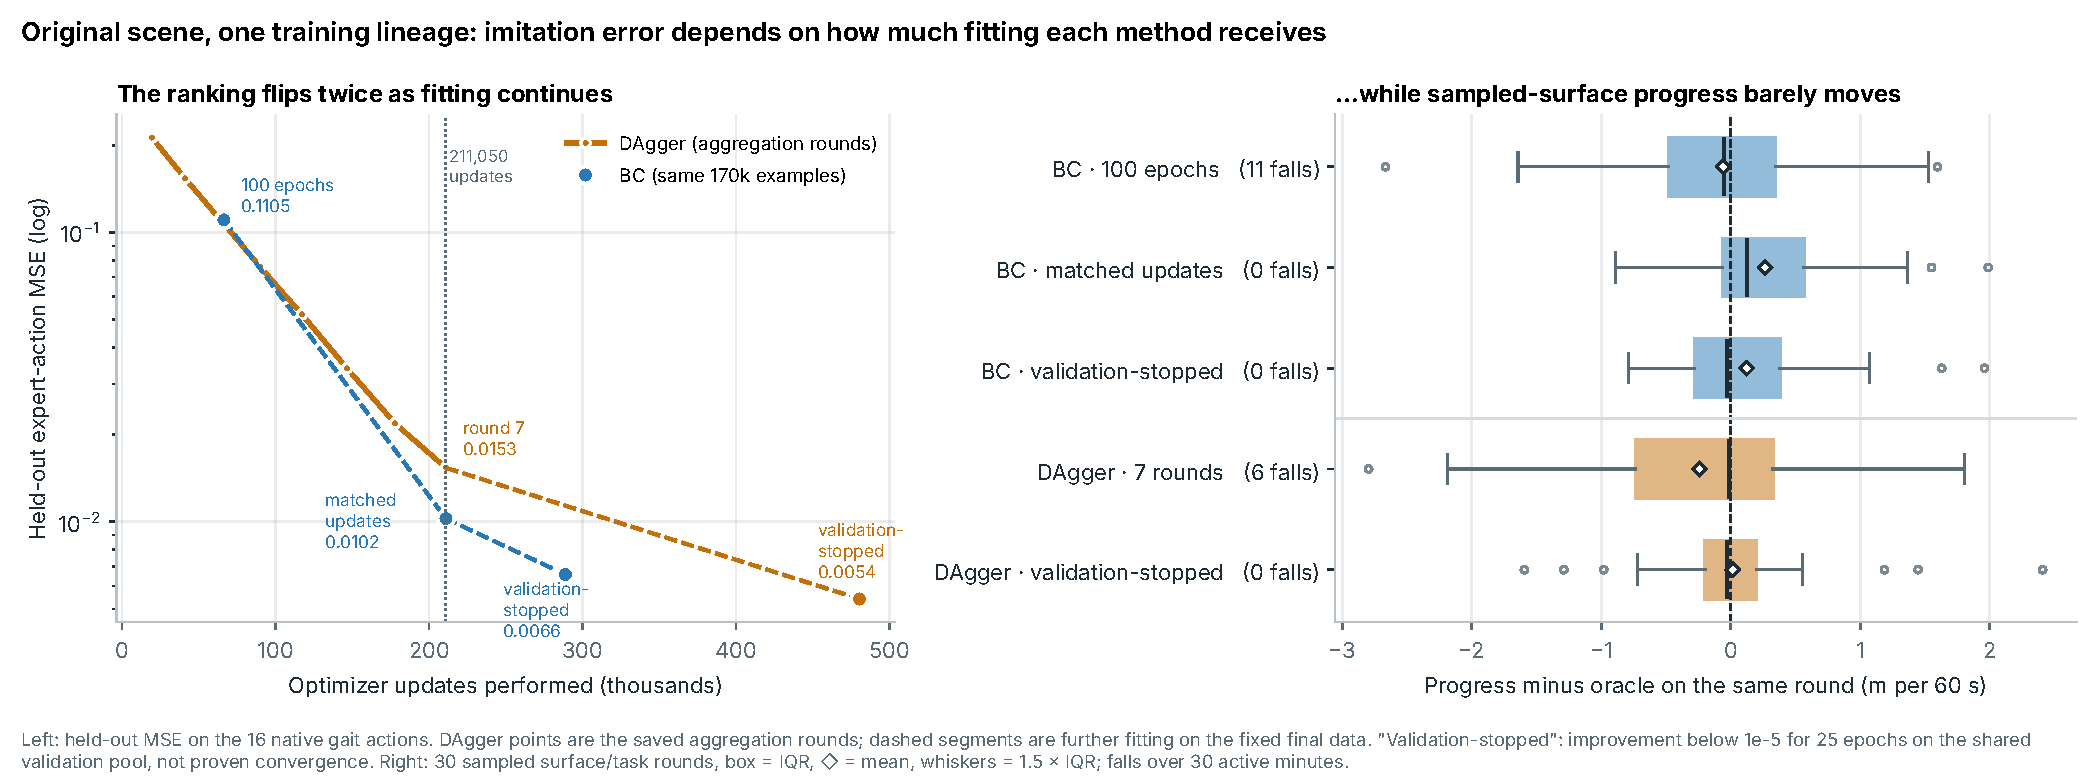
\includegraphics[width=\textwidth]{fig1_allocation.pdf}
\caption{Original field, one training lineage. Left: held-out action error against optimizer updates performed. The BC--DAgger ranking reverses twice as fitting continues. Right: paired progress difference from the expert on the 30 altered-surface rounds; box = interquartile range, line = median, $\diamond$ = mean, whiskers = 1.5$\times$IQR; falls over 30 active minutes.}
\label{fig:allocation}
\end{figure*}

Figure~\ref{fig:allocation} and Table~\ref{tab:original} show the central result. At the initial fixed budgets, DAgger's held-out error (0.0153) is 7.2$\times$ lower than BC's (0.1105). That budget gave BC 66,500 updates against DAgger's 211,050. At matched updates BC's error falls to 0.0102, 33.3\% below DAgger's, and its on-policy error (0.0040) is also lower than DAgger's (0.0078). At nearby update counts on the learning curves the two methods differ by 0.5\% (BC 0.1105 at 66,500 updates, DAgger 0.1100 at 64,500). Under the common validation-stopping rule DAgger has lower error: 0.0054 against 0.0066 (17.7\% lower held-out, 8.2\% lower on-policy), with 480,375 performed updates compared with BC's 288,855 (66.3\% more).

\begin{table}[t]\centering\small
\caption{Original field, mean of five deployments. MSE is over the 16 gait actions; progress in metres per 60\,s.}
\label{tab:original}
\setlength{\tabcolsep}{3pt}
\begin{tabularx}{\columnwidth}{lRRRR}\toprule
Controller & Updates & Held-out MSE & On-policy MSE & Progress \\
\midrule
Expert & --- & --- & 0 & 44.45 \\
BC, initial & 66,500 & 0.1105 & 0.0744 & 44.63 \\
BC, matched & 211,050 & 0.0102 & 0.0040 & 43.91 \\
BC, val.-stopped & 288,855 & 0.0066 & 0.0021 & 44.17 \\
DAgger, 7 rounds & 211,050 & 0.0153 & 0.0078 & 44.36 \\
DAgger, val.-stopped & 480,375 & 0.0054 & 0.0019 & 43.98 \\
GAIL-BC & BC + PPO & 0.1104 & --- & 44.56 \\
GAIL-DM & DAgger + PPO & 0.0157 & --- & 44.15 \\
\bottomrule\end{tabularx}
\end{table}

Each of these three statements is a correct description of a different allocation. None of them identifies an intrinsically better algorithm. The right panel of Figure~\ref{fig:allocation} shows the corresponding task progress on altered surfaces: mean paired differences from the expert range from $-0.24$\,m (seven-round DAgger) to $+0.27$\,m (matched BC), that is, $-0.7$\% to $+0.8$\% of the expert's mean progress.

The varied-surface comparisons also change after additional fitting (Figure~\ref{fig:varied}). After their initial training, continued hidden BC had 10.7$\times$ DAgger's held-out error, and across the four paired BC--DAgger comparisons (eight model families) BC's deficit was 4--11$\times$. After validation-stopped fitting it is 0.9--1.1$\times$, and for the input-conditioned continued models BC's error is the lower of the two. Additional fitting duration differs: continued DAgger stopped after 25--70 further epochs (two replicas selected their starting checkpoint), whereas continued BC stopped after 217--448.

\begin{figure*}[t]\centering
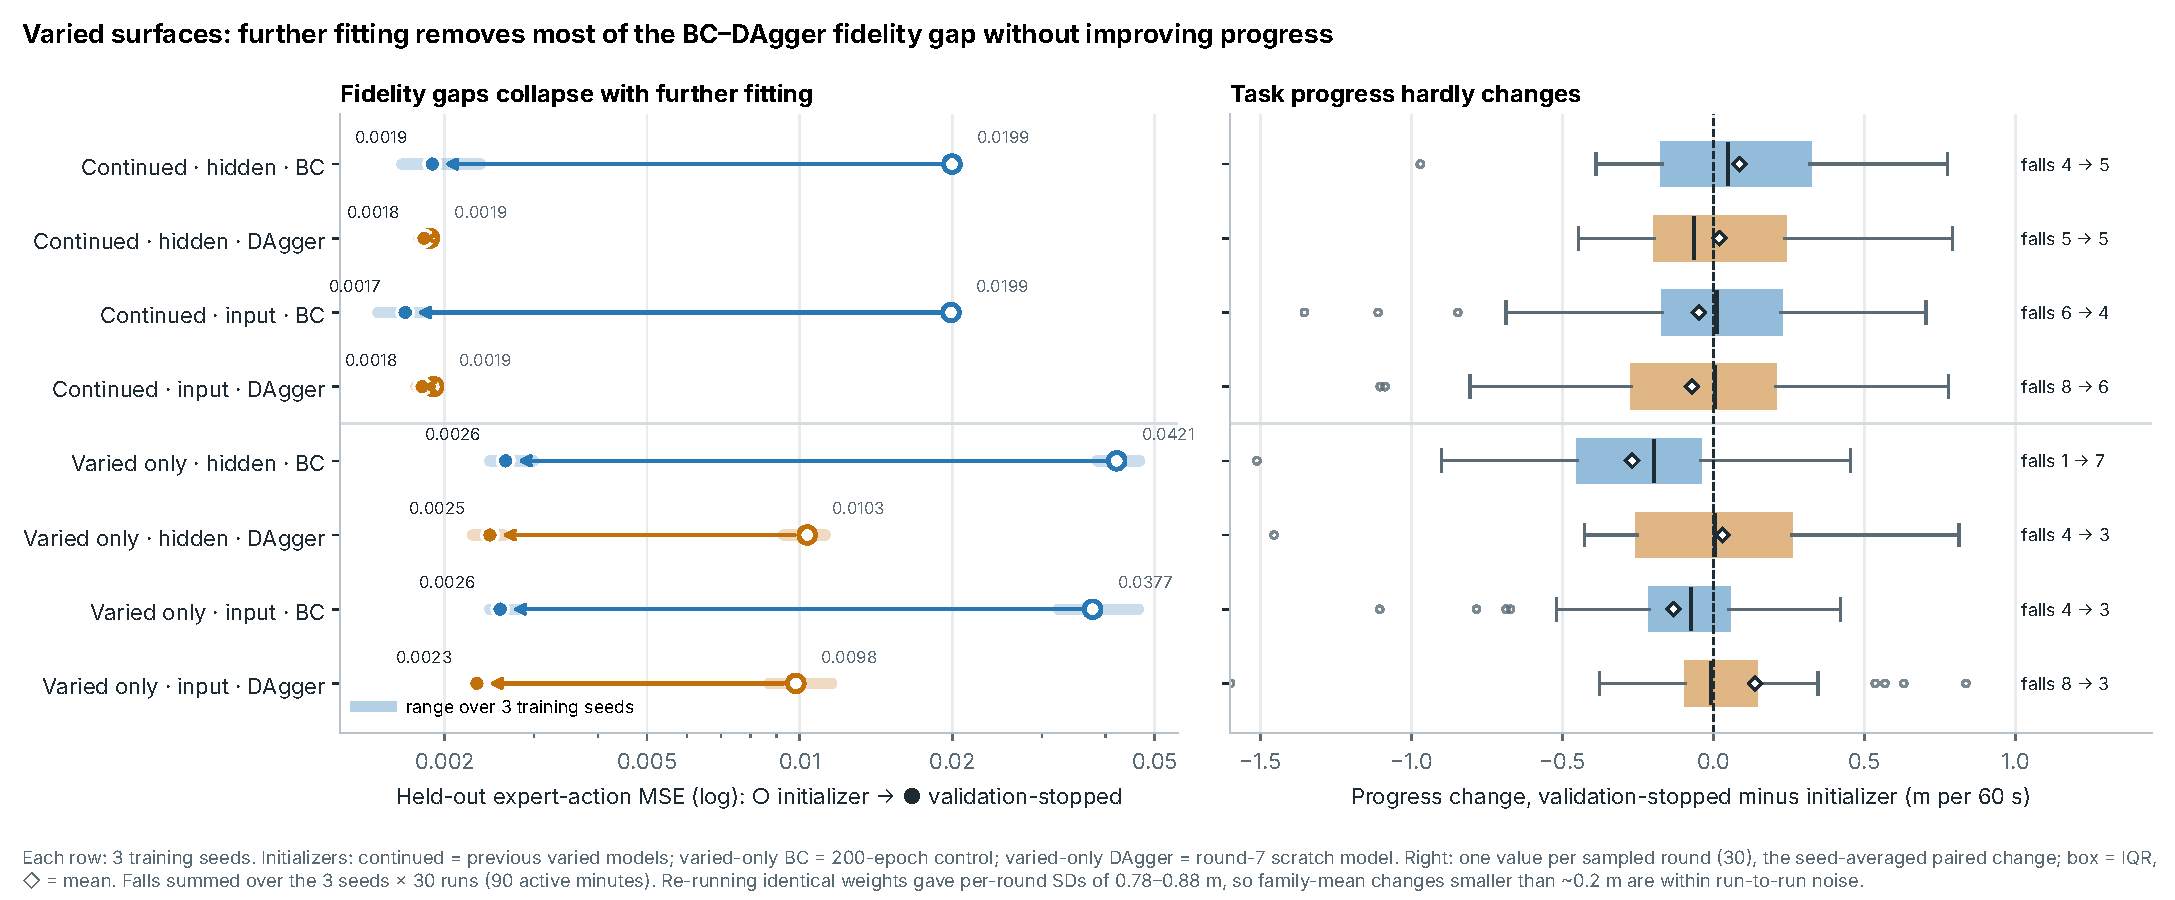
\includegraphics[width=\textwidth]{fig2_varied.pdf}
\caption{Varied-surface families, three training seeds each. Left: held-out error before ($\circ$) and after ($\bullet$) validation-stopped fitting. Right: paired change in progress on the 30 altered-surface rounds; falls summed over 90 active minutes. Intervals describe uncertainty across the sampled rounds conditional on the trained checkpoints, not across new training histories (Section~\ref{sec:measurement}).}
\label{fig:varied}
\end{figure*}

From a supervised start, GAIL refinement changed held-out error by $-0.05$\% for GAIL-BC (0.11047 to 0.11042) and $+2.4$\% for GAIL-DM (0.01535 to 0.01572; Table~\ref{tab:original}). Median paired progress differences between each GAIL model and its initializer lie within $\pm0.11$\,m, and all eight varied-family intervals include zero. From a random start, 70,000 steps produced no walking (progress $-0.12$\,m on the original field and $-0.37$\,m for the varied-hidden variant, no targets reached). RobocupGym reports reinforcement-learning baselines trained for 5 million steps \citep{beukman2024}; those tasks and training objectives differ, so this is contextual information rather than a matched-budget comparison.

The two tested DAgger seed-dataset configurations produced different errors. A first DAgger implementation started from 20,000 expert examples. Replacing that seed with 100,000 balanced examples, with the same seven rounds and $\beta$ schedule, reduced held-out error by 78.5\% and on-policy error by 95.0\%. This change altered both the size and the composition of the seed, so the two cannot be separated.

\subsection{RQ3: comparison with the expert}

On the original field, mean progress of the seven supervised-initialized learners ranges from 43.91 to 44.63\,m against the expert's 44.45\,m ($-1.2$\% to $+0.4$\%), and forward velocity from 0.747 to 0.762\,m/s against 0.759\,m/s ($-1.6$\% to $+0.4$\%; Table~\ref{tab:original}). On the altered-surface suite, means of the 33 supervised-initialized model families (averaged over training seeds) range from 32.50 to 33.30\,m against the expert's 32.89\,m ($-1.2$\% to $+1.3$\%); individual seed models range from 32.50 to 33.49\,m ($-1.2$\% to $+1.8$\%).

The tested zero-action and untrained-network controls do not reproduce this useful walking through the gait engine (Figure~\ref{fig:engine}). With zero actions the robot makes $-0.30$\,m of progress on the altered-surface suite; three untrained networks make $-0.16$, $-0.64$ and $-0.27$\,m; uniform random actions fall 704 times in 30 minutes. Fall counts alone do not distinguish these outcomes: on the original field, the zero-action controller and the untrained networks recorded no falls while making no progress.

\begin{figure*}[t]\centering
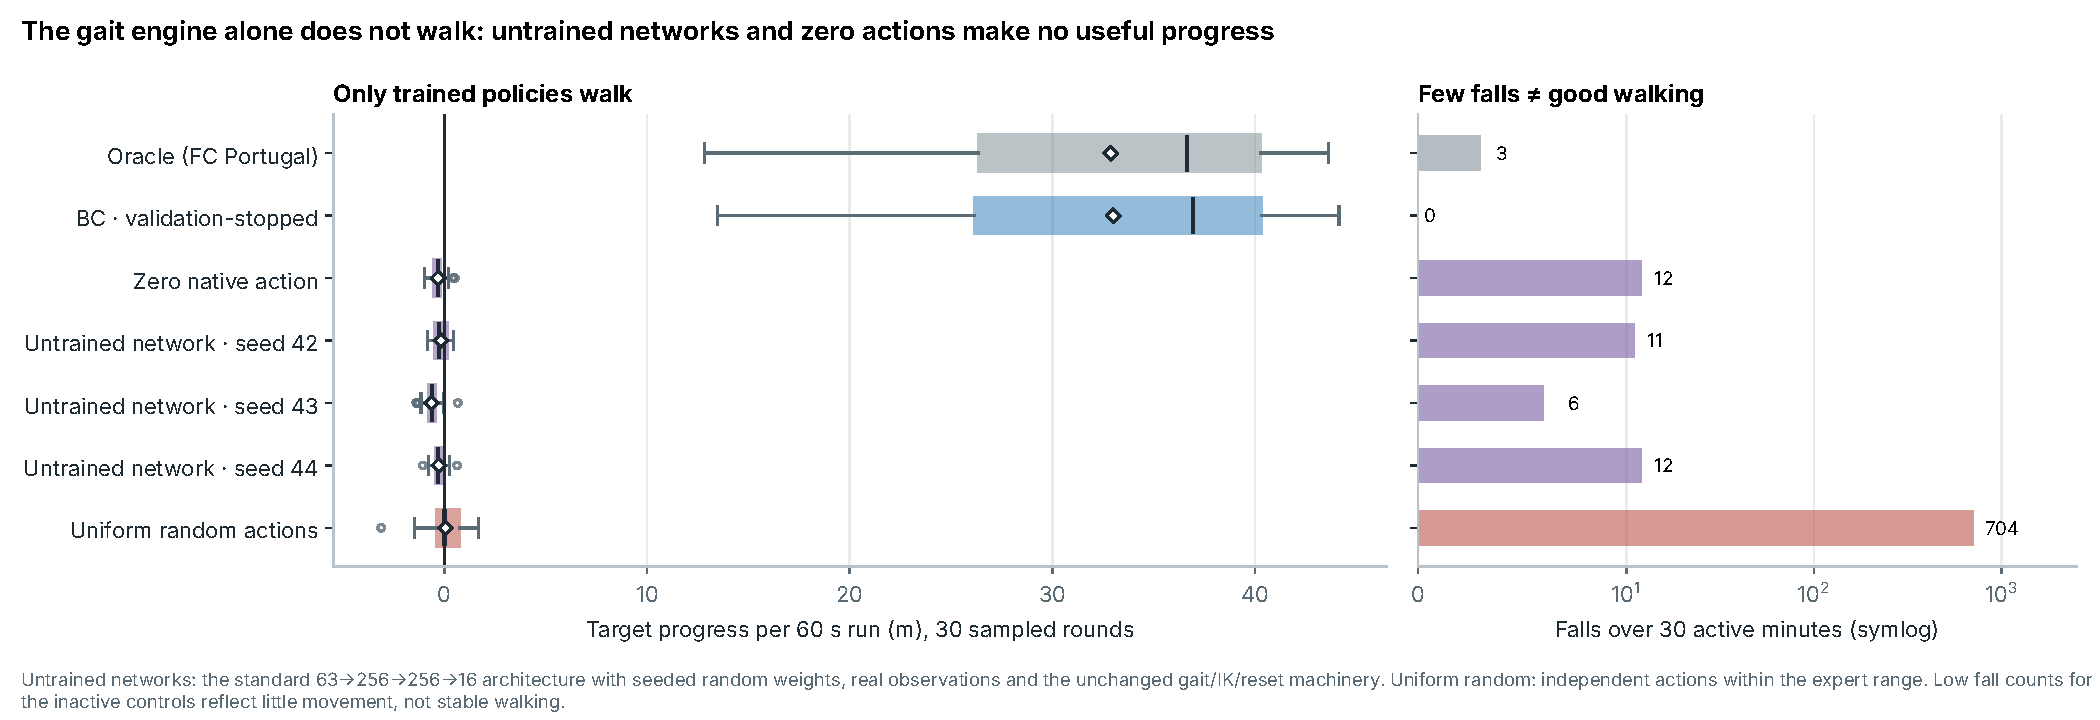
\includegraphics[width=\textwidth]{fig3_engine.pdf}
\caption{Engine controls on the 30 altered-surface rounds. The same gait generator, inverse kinematics and resets driven by zero actions, untrained networks or random actions make no useful progress. Fall counts should be interpreted alongside progress because the controls differ substantially in movement.}
\label{fig:engine}
\end{figure*}

Lower action error was not accompanied by higher progress. Varied-only hidden BC reduced its held-out error by 93.7\% under validation stopping, while its mean progress decreased by 0.27\,m per 60\,s [$-0.38$, $-0.17$] and recorded 7 rather than 1 fall over 90 minutes. Varied-only input BC had a mean progress decrease of 0.13\,m [$-0.23$, $-0.03$]. These observed progress losses are under 1\% and their conditional intervals exclude zero. They show that improved action fidelity need not coincide with improved progress for these checkpoints. The sparse fall counts and limited replication do not establish a general effect of further fitting on balance or control. Among policies trained on the original field, validation-stopped DAgger made 0.11\,m less progress than validation-stopped BC on the altered-surface suite [$-0.26$, $+0.04$], despite its lower action error. Matched-update BC had a smaller observed lower-tail deficit: the mean of the three worst paired deficits is $-0.66$\,m for matched BC against $-1.92$\,m for initial BC and $-2.38$\,m for the seven-round DAgger.

\subsection{RQ1: stability}

\begin{figure}[t]\centering
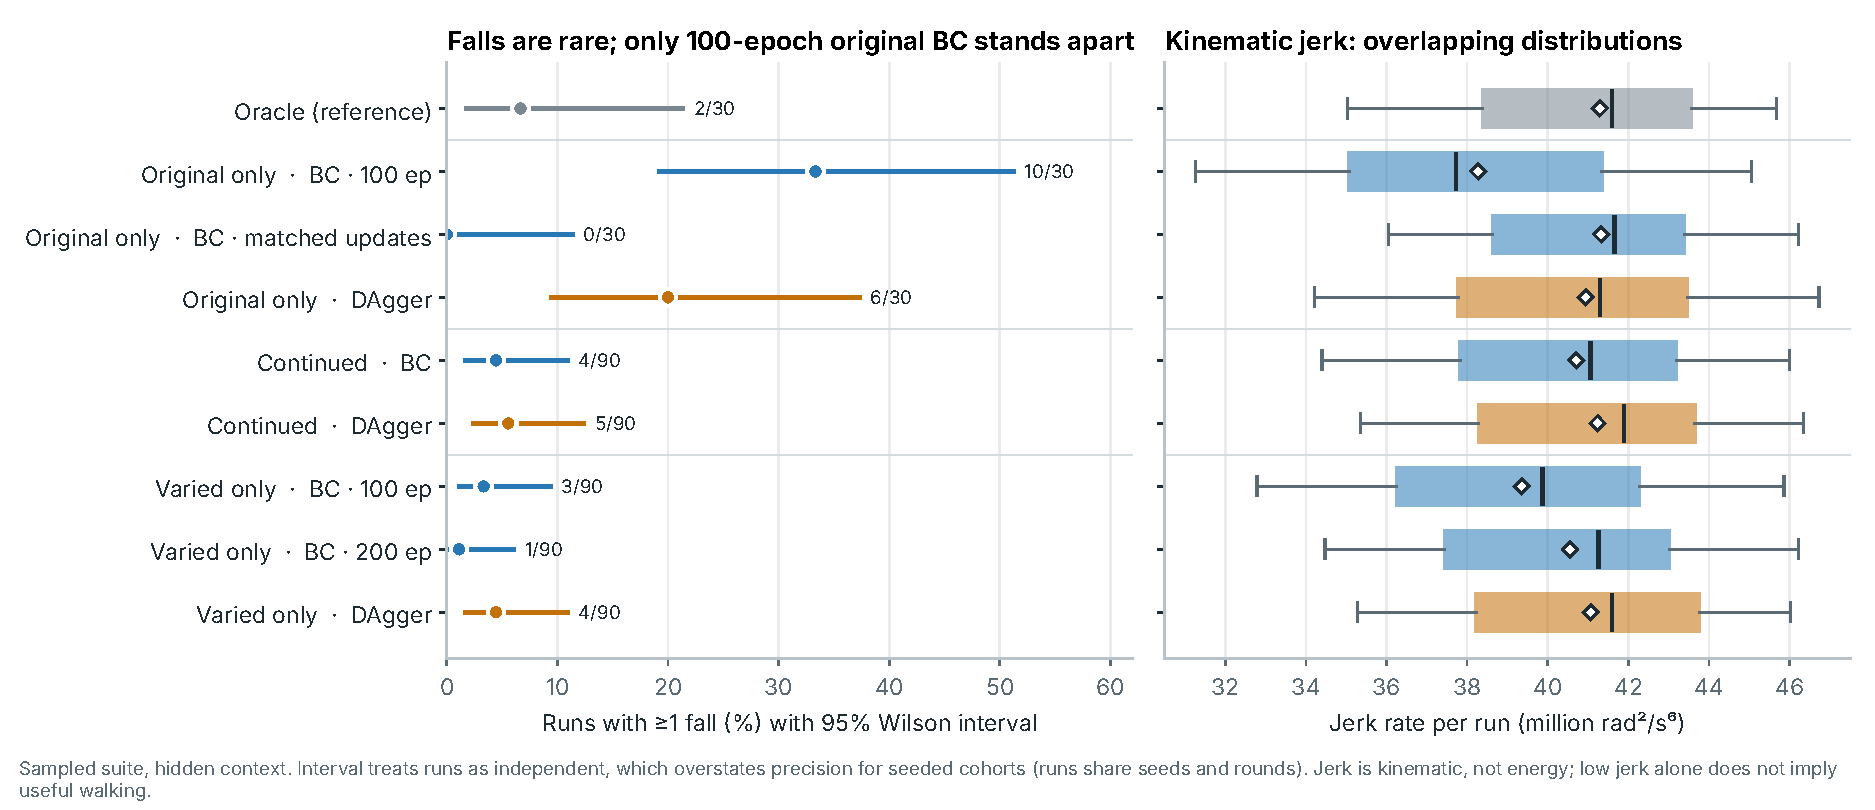
\includegraphics[width=\columnwidth]{fig4_stability.pdf}
\caption{Stability of fixed-budget models on the altered-surface suite (hidden-context models). Left: share of runs with at least one fall; displayed Wilson intervals assume independent runs. Shared rounds and training histories limit this assumption, so the intervals are descriptive and their overlap is not a test of method differences. Right: kinematic jerk rate per run.}
\label{fig:stability}
\end{figure}

We did not resolve a consistent stability advantage across the tested methods and allocations (Figure~\ref{fig:stability}). Initial 100-epoch BC fell in 10 of 30 altered-surface runs (33.3\%; 11 falls), against none for matched-update BC. These checkpoints share the same data, architecture and initialization, so additional fitting is associated with improved observed stability within this lineage; this is not an independently replicated estimate of its effect. After validation stopping, both original-field models recorded no falls on the altered-surface suite, and varied families recorded 3--7 falls per 90 minutes. During training, mixed-DAgger collection never fell in 910,000 steps (including the rounds with $\beta=0$).

Progress and jerk were associated in the evaluated runs. Across the 26 extended policies and their 30 shared rounds, progress and jerk are strongly correlated (Spearman $\rho=0.93$); after removing each round's mean the correlation falls to 0.32, indicating that the pooled association depends strongly on the shared round conditions. Within rounds, action error and jerk are negatively correlated ($\rho=-0.77$), and under-fitted BC damps 9 of its 16 actions by 2--6\%. The measured change in action damping was not significantly associated with progress changes after further fitting ($\rho=-0.19$, permutation $p\approx0.39$, 24 pairs).

\subsection{GAIL before and after the training changes}
\label{sec:gail}

\begin{figure*}[t]\centering
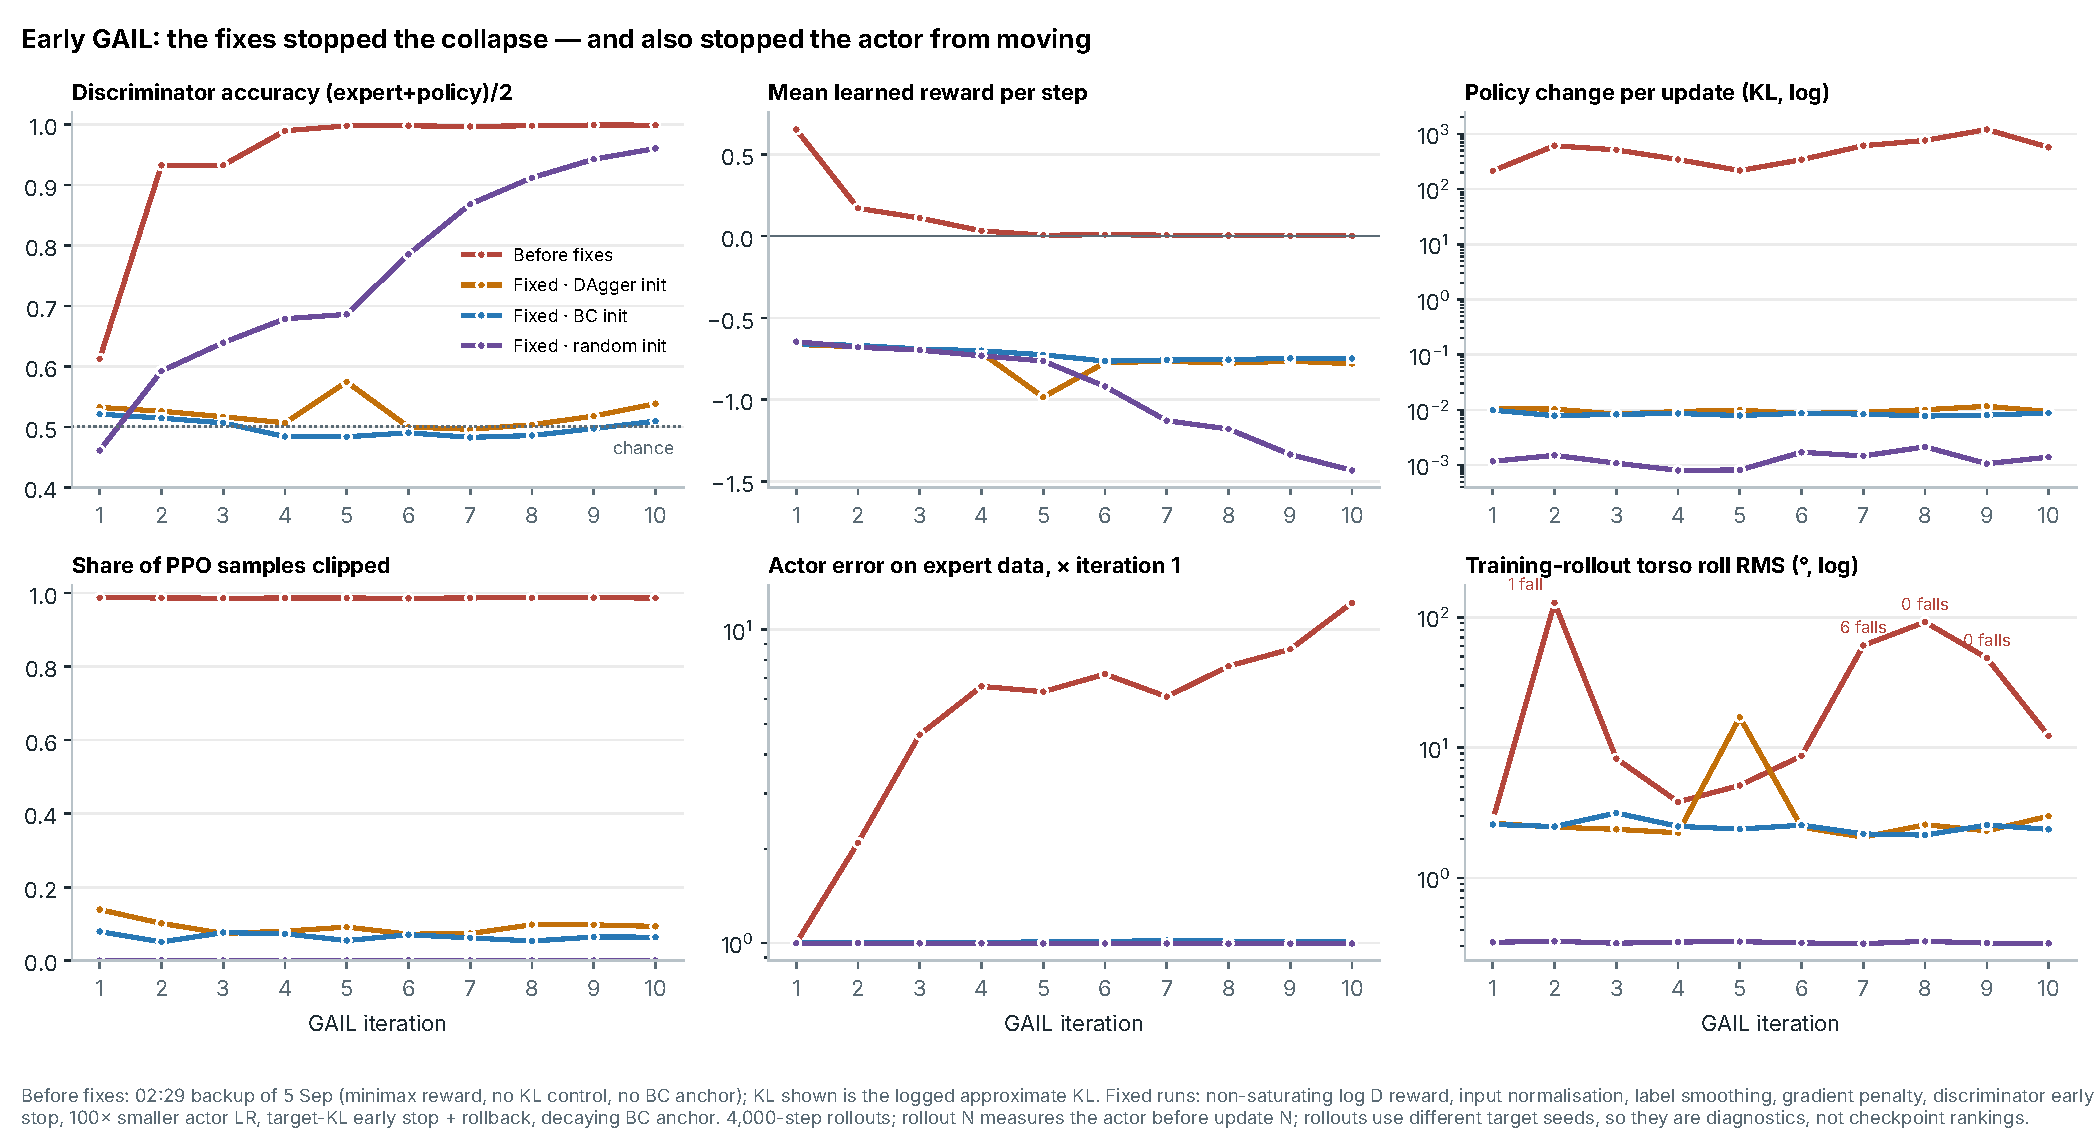
\includegraphics[width=\textwidth]{fig5_gail.pdf}
\caption{GAIL training before and after the changes to its reward and update rules (4,000-step rollouts; diagnostics, not checkpoint rankings). Before the changes, discriminator accuracy approached 1, the learned reward approached 0, approximate KL per update reached $10^2$--$10^3$ and actor error on expert data grew. After the changes, the supervised-initialized actors' error on expert data varied by at most 2\% across ten iterations, and the random-initialized actor reached no targets.}
\label{fig:gail}
\end{figure*}

The initial reported GAIL implementation, initialized from DAgger with the minimax reward and no KL control, diverged (Figure~\ref{fig:gail}). Over ten iterations the discriminator's balanced accuracy rose from 0.61 to 0.999, the mean learned reward fell from 0.65 to 0.0017, approximate KL per update was 215--1,203 with 98.6--98.7\% of PPO samples clipped, actor error on expert data rose from 0.87 to 10.6 (12.2$\times$), and the robot ended up toppled. After the changes listed in Section~\ref{sec:learners}, the discriminator's balanced accuracy stays between 0.48 and 0.57, accepted KL stays between 0.0077 and 0.0116 without rollbacks, and the actor's error on expert data stays within 0.2678--0.2683 (DAgger-initialized run) and 0.00705--0.00719 (BC-initialized run) over ten iterations. The reported random-initialized run did not show the earlier divergence, but reached no targets: its discriminator's balanced accuracy rises from 0.46 to 0.96 while KL stays at 0.0008--0.0021, its error on expert data changes from 7.69 to 7.65, and it reaches no targets.

All changes were introduced together, so we cannot attribute either the absence of divergence or the small changes in expert-data error of the supervised-initialized actors (at most 2\% change in error on expert data) to any single change. Several of the changes (the BC loss, the smaller actor learning rate and the KL limit) penalize deviations or constrain the size of parameter updates. Their individual effects were not measured.

\subsection{Altered surfaces and explicit context}

\begin{figure*}[t]\centering
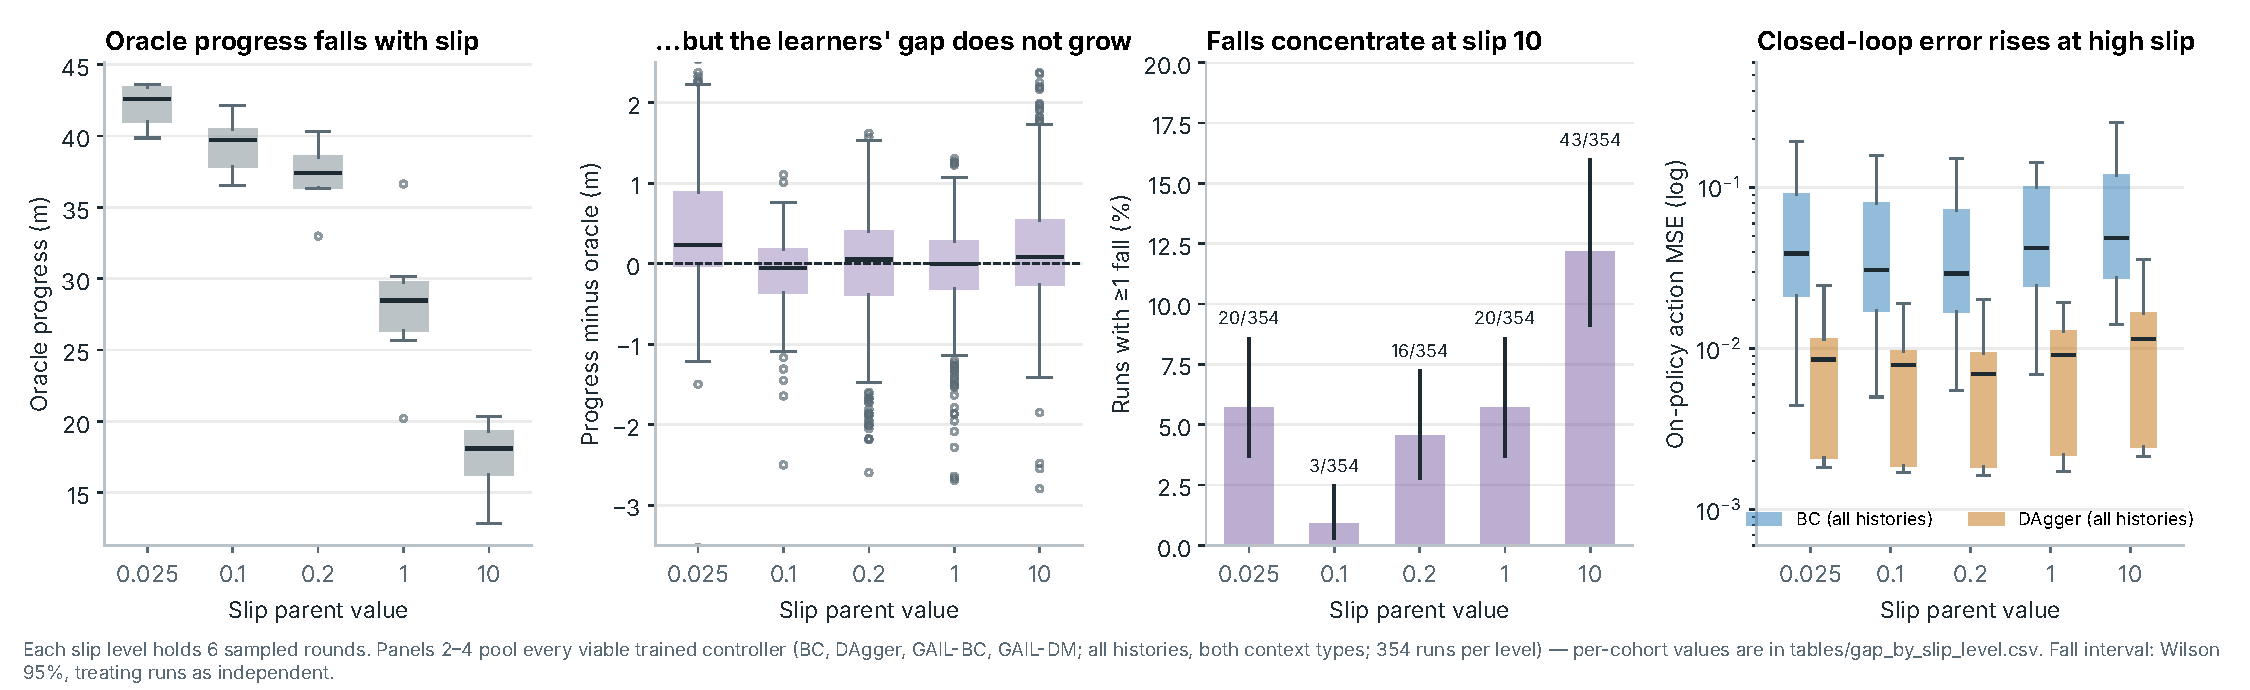
\includegraphics[width=\textwidth]{fig6_surfaces.pdf}
\caption{Altered surfaces, grouped by the slip value each round was drawn around (six rounds per level; learner panels pool the trained BC, DAgger and GAIL controllers, 354 runs per level). Rounds vary the target sequence as well as slip, so this is not an isolated slip-response curve.}
\label{fig:surfaces}
\end{figure*}

At higher slip values both the expert and the learners progressed less (Figure~\ref{fig:surfaces}). The expert's median progress falls from 42.6\,m at the lowest slip level (0.025) to 18.1\,m at slip 10, while the learners' paired gap stays centred near zero at every level. Differences between these groups also occur in falls (43 of 354 runs with a fall at slip 10, against 3 of 354 at slip 0.1) and as higher on-policy action error.

Providing the slip value as an input did not produce a consistent progress advantage across the tested families. After validation stopping, input-minus-hidden progress intervals include zero for three of four families; the exception, varied-only BC ($+0.19$\,m [$+0.07$, $+0.32$]), coincides with the progress decrease of the hidden model after further fitting and is not corrected for multiple comparisons. In an earlier BC study (90 paired runs), supplying a wrong slip value (10 on surfaces with slip at most 0.5, otherwise 0.025; median ratio to the actual slip 93$\times$) changed median on-policy error by $+1.3$\%, mean progress by $+0.01$\,m and the fall count not at all (4 against 4), indicating small changes in these measured outcomes under the tested input substitutions. \citet{beukman2023} note that a context-unaware policy can perform well when the same policy makes progress in every context; here the expert has no slip input and makes progress on every tested surface.

\subsection{Representations}
As an exploratory extension, we asked whether accessible information in hidden features helps explain the fidelity and task-performance differences. We fitted linear ridge probes \citep{alain2016} on a shared bank of oracle trajectories, using ten runs for fitting, five for penalty selection and fifteen for testing; scaling used fitting data only. The study covered 131 representations and 30 targets, with raw-input, random-network and three shuffled-label controls \citep{hewitt2019}, alongside CKA comparisons \citep{kornblith2019}. Future targets describe outcomes under oracle actions, not each learner's deployment. These examples do not show a consistent correspondence between probe scores and deployment performance. The untrained networks that cannot walk decode command displacement with $R^2=0.97$. DAgger's phase--roll probe score decreases (0.712 to 0.694) while its action error falls by 65\%, and its hidden layers keep a CKA of 0.99 with its initializer through that change. We use these results only descriptively.

%======================================================================
\section{Discussion}

\subsection{The choice of standardised resource}
The tested BC, DAgger and GAIL configurations have different resource requirements, and our allocations do not equalize all of them (Table~\ref{tab:resources}). The three standardisations we used give three different fidelity rankings: DAgger 7.2$\times$ lower held-out error, BC 33.3\% lower, and DAgger 17.7\% lower at 66.3\% more updates. Under all three, mean paired progress was within $-0.7$\% to $+0.8$\% of the expert's. Prior comparisons also fixed different resources for different methods: \citet{ho2016} matched environment interaction among adversarial methods but validation-stopped their BC baseline, and \citet{ross2011} compared methods per collected label. In our study, further supervised fitting substantially changed action MSE and the BC--DAgger ranking. Inherited costs are a further unequal quantity: GAIL inherits its initializer's demonstrations, updates and (for GAIL-DM) expert queries, and continued models inherit their original-field training.

For RQ2, the cited DAgger study reports comparisons against collected labels \citep{ross2011}, whereas the cited GAIL study controls environment interaction for several methods \citep{ho2016}. We do not assign a common cost conversion to labels, simulator steps and optimizer updates. Our expert is programmatic, so the human feedback that \citet{celemin2022} use to measure the efficiency of interactive methods was not incurred. We report outcomes at the tested allocations and fitting curves, not normalized-return learning curves against queries or environment steps. These results describe outcomes at the recorded resource allocations; they do not establish general sample-complexity rates.

We suggest that comparisons of imitation methods state which resource is held fixed, account for inherited costs, and show results under more than one standardisation, or as outcome-against-cost curves, since here the choice of standardisation changed the fidelity ranking.

\subsection{Relation to conditions identified in prior work}
Changing the fitting allocation changed the observed fidelity ranking, while mean task progress remained close across methods. Prior work provides possible explanations, but our experiments do not identify a mechanism. \citet{spencer2021} discuss realizability of the expert within the learner's policy class. Our expert has one 64-unit tanh layer and the learners have two 256-unit ReLU layers; this architecture comparison alone does not establish realizability. \citet{ho2016} report satisfactory BC performance with sufficient data on several locomotion tasks. Our BC training set contains 170,000 examples, but we did not systematically vary its size, so we cannot identify a data-sufficiency threshold. \citet{ross2011} relate their performance bounds to the cost of errors and recovery conditions. We did not measure recovery to the expert's state distribution. The observed absence of falls during mixed-DAgger collection and the action-error ratios reported here do not establish that condition.

The study also contains comparisons involving different initial datasets or training budgets: DAgger with a 20,000-example seed, BC at 100 epochs, and GAIL from random weights with 70,000 steps. \citet{ho2016} report the opposite outcome on their Humanoid task, where BC did not exceed 60\% of expert performance and GAIL matched the expert. Their policies act directly on the simulator's joint actuators, whereas ours act through a gait generator; whether this difference in interface accounts for the different outcome was not tested.

The GAIL result applies to the tested recipe, which changed its initializer's held-out action error by at most 2.4\%. Learning from few demonstrations, the setting in which \citet{ho2016} report GAIL's advantage over BC, was not tested.

\subsection{Limitations}
The original-field comparison has a single training lineage, and continued varied families share original-field parents across their three seeds, so those seeds are not independent complete training histories. Wall-clock time, expert compute and repeated training were not equalized. Validation stopping is not convergence, and validation-stopped DAgger collected no new labels. Our expert supplies programmatic labels without human annotation noise; \citet{celemin2022} note that most interactive methods ``have been evaluated with unrealistic perfect oracles''. Rounds vary target sequences together with slip, so slip effects are not isolated. Jerk is kinematic, not torque. The wrong-context test covers BC only. Many contrasts are exploratory and uncorrected for multiplicity, and confirmation rounds had been examined before probing. All results are in simulation, for one skill and one robot model.

\subsection{Future work}
No further experiments were run for this paper. Three directions follow. First, experiments varying the BC-loss weight, actor learning rate and interaction budget separately could test their effects on GAIL refinement. Second, settings without the properties discussed above would test whether the methods then differ: fewer or imperfect demonstrations, an expert of greater capacity than the learner, external pushes, raw joint control without the gait generator, or other skills such as kicking or getting up. Third, the context result should be checked with wrong-context evaluation for all algorithms, and comparisons should report outcomes against each cost axis (demonstrations, expert queries, environment steps, optimization and wall-clock time).

%======================================================================
\section{Conclusion}
On RoboCup 3D walking through FC Portugal's gait interface, every BC, DAgger and BC-anchored GAIL learner's mean progress was within 1.8\% of the expert's, and no consistent stability advantage was resolved across the tested methods and allocations. The methods' imitation fidelity ranking depends on which resource is held fixed and reverses twice across three standardisations. After changes to its reward and update rules, GAIL refinement changed its initializer's held-out action error by at most 2.4\%. These findings are restricted to the tested walking task, interface, datasets and training configurations. The experiments do not establish why mean progress remained similar across methods or how the ranking would change in other settings. We recommend that such comparisons report which resource they standardise and show results under more than one choice.

\section*{Data and reproducibility}
All results come from saved checkpoints and evaluation receipts; no checkpoint was selected using test data. The figures and numbers in this paper are produced by scripts in the project repository from versioned summary files, together with a reproduction guide. Repository and archive links are to be added before submission.

\label{bodyend}
\clearpage
\bibliographystyle{plainnat}
\bibliography{references}
\end{document}
